% TeX-command-default: "LaTeX"
\documentclass[12pt,french]{article}
\usepackage[utf8]{inputenc}
\usepackage[T1]{fontenc}
\usepackage{babel}
\usepackage{graphicx}
\usepackage{float}
\usepackage{csquotes}
\usepackage{epigraph}
\usepackage{wrapfig}
\usepackage{rotating}
\usepackage[normalem]{ulem}
\usepackage{amsmath}
\usepackage{textcomp}
\usepackage{amssymb}
\usepackage{capt-of}
\usepackage{lmodern}
\usepackage{hyperref}
\usepackage[margin=1.4in]{geometry}
\usepackage{parskip}
\usepackage{microtype}
\usepackage{gatin} % Personnal styling


\author{SUBLET Gary -- 11506450 \\[.3em] VILLERMET Quentin -- 11507338}
\date{\today}
\title{Intelligence Bio-Inspirée \\[.5em] Travaux Pratiques}

\begin{document}

\gatintitle{Compte-rendu des travaux pratiques sur l'apprentissage profond par renforcement}

\tableofcontents
\newpage

\section{Réplicabilité}
\subsection{Environnement virtuel}

La totalité des expérimentations suivantes ont été réalisées avec Python 3.7, au sein de \textit{notebooks jupyter} et de scripts \textit{.py}.

Afin de favoriser la facilité de reproduction de ces programmes, nous évoluons dans un environnement virtuel, où les modules python peuvent être plus aisément contrôlés. \\
Nos dépendances sont listées dans le fichier \texttt{requirements.txt} à la racine du projet.

Un guide permettant la mise en place de ce \textit{virtualenv} est présent dans le \texttt{Readme.md} du dépôt GitHub.

\section{Deep Q-network sur CartPole}
\subsection{Début}
\subsubsection{Question 1 -- Agent aléatoire CartPole-v1}

Le code de l'agent aléatoire est entièrement contenu dans le fichier \texttt{cartpole.py}, trouvable dans les sources du projet.

Il est presque entièrement basé sur l'exemple des créateurs de \texttt{gym} présent sur le \href{https://github.com/openai/gym}{GitHub} du module.

\subsubsection{Question 2 -- Évaluation des récompenses}

\begin{note}
En plus de l'affichage demandé, nous avons pris l'initiative de créer une visualisation de la récompense cumulée au fil des épisodes (dénotant en quelque sorte le \og succès\fg\, de la session d'apprentissage.
\end{note}

Nous avons opté pour un affichage \texttt{matplotlib}, avec \textit{mean-pooling} pour alléger le graphe en cas de grand nombre d'épisodes lorsque nécessaire.

Dans notre premier cas, soit celui d'un agent aléatoire sur l'environnement \textit{CartPole-V1}, le graphe des récompenses cumulées en fonction du nombre d'interactions aboutit forcément à un nuage de points suivant la fonction $f(x) = |x|$.

On constate peu d'\textit{outliers} (qu'on considèrera ici comme ayant $x > 60$), en raison du caractère aléatoire des décisions.

\seprule{19.12.2019}
\begin{center}
    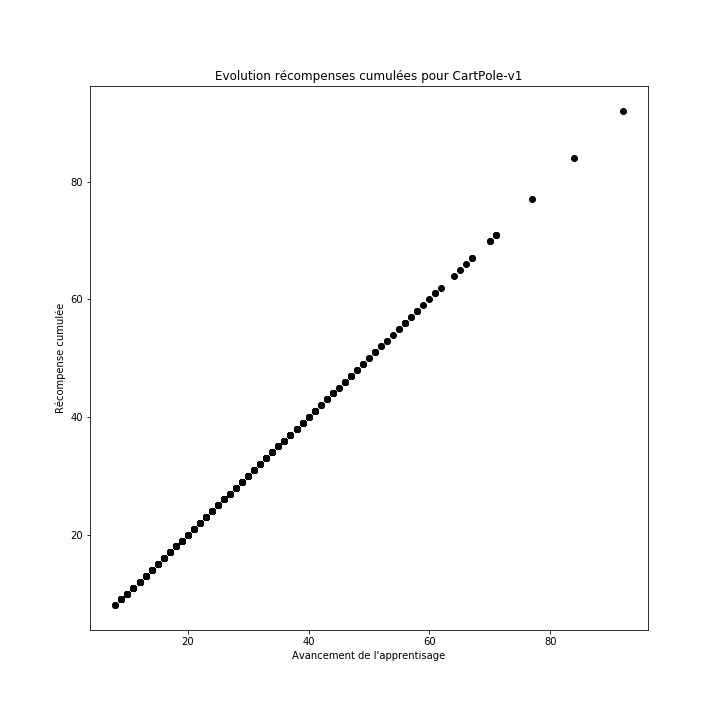
\includegraphics[width=\textwidth]{../src/img/env_CartPole-v1_random_cumu.png}
\end{center}

Ce résultat est sans surprise, puisque toute interaction entraîne une récompense de 1 dans cet environnement.

La deuxième visualisation n'est pour le moment pas très utile non plus, puisque notre agent n'apprend pas et agit de façon aléatoire.

\begin{center}
    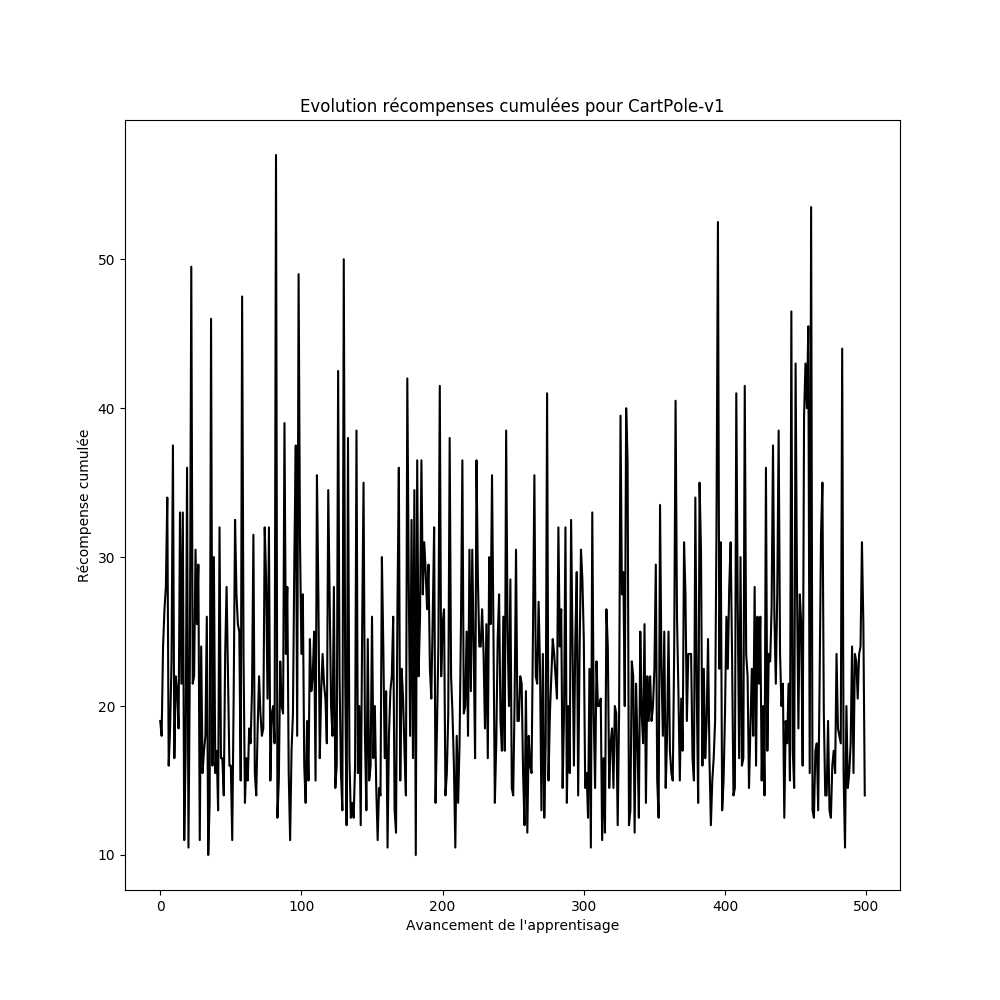
\includegraphics[width=\textwidth]{../src/img/env_CartPole-v1_random.png}
\end{center}

Ces deux affichages prendront leur pertinence plus tard dans le développement, lorsque notre agent commencera à apprendre de son environnement.

Il nous indiqueront respectivement la rapidité d'apprentissage des épisodes individuels, et l'efficacité générale de l'apprentissage en fonction du temps passé (\textit{i.e.} des épisodes).

\newpage
\subsection{Experience replay}

\subsubsection{Question 3 -- Buffer de stockage d'expériences}

Le code du buffer \textit{experience replay} est dans le fichier \texttt{deeprl\_agent.py}, plus particulièrement la fonction \texttt{experience} de la classe \texttt{Agent}.\\
Cette question marque le début du code des notebooks jupyter.

\subsubsection{Question 4 -- Sampling de mini-batch}

À partir de cette question, nous basculons sur un système de notebooks \textit{Jupyter} pour une implémentation plus rapide des tests. \\
La récupération de mini-batch de données du buffer se fait donc dans le fichier \texttt{experience\_replay.ipynb}.

\subsection{Deep Q-learning}

L'implémentation du Q-learning se fait dans la continuation de la partie précédente, donc dans le fichier \texttt{experience\_replay.ipynb}. Sauf indication du contraire, c'est au sein de ce notebook que le reste du TP se déroulera.

\subsubsection{Question 5 -- Réseau de neurones}

Pour notre premier exemple, on construit donc un réseau avec 4 neurones d'entrée et 2 neurones de sortie.

En effet, dans l'environnement \textit{CartPole-v1}, l'observation est de type \texttt{Box(4,)} et le domaine des actions est un \texttt{Discrete(2)} (en l'occurence 0 et 1 pour bouger à gauche et à droite respectivement).

Ces dimensions expliquent la taille de notre réseau.

\subsubsection{Question 6 -- Approximation des Q-valeurs}

Les deux stratégies d'exploitation proposées sont implémentées dans la classe \textit{Agent}, qui est dotée des fonctions \texttt{epsilongreedy(self, ob, epsilon)} et \\\texttt{boltzmann(self, ob, tau)} qui renvoient l'action choisie, qui est soit une action aléatoire d'exploration, soit le choix déterminé par la politique d'après les Q-valeurs prédites par le réseau.

Pour la politique $\epsilon$-greedy, il s'agit de la meilleure action avec une probabilité $(1 - \epsilon)$. Pour Boltzmann, le choix est stochastique mais tend malgré tout à choisir la Q-valeur maximale le plus souvent.

\subsubsection{Question 7 -- Apprentissage}

À ce stade du développement, notre agent utilise désormais toute une panoplie de fonctions ; à chaque fois qu'il doit choisir une action, il fait appel à \texttt{choose\_action(ob, reward, done)}, qui détermine les Q-values avant de déterminer (selon la méthode d'exploration actuelle) l'action choisie.

Après avoir effectué son action, celle-ci est appliquée à l'environnement par le biais de la fonction \texttt{step()}, après quoi on fait appel à l'\textit{experience replay}. Pour ce faire, on utilise la fonction \texttt{experience()} de la classe \textit{Agent.}

À la fin de notre épisode, on utilise \texttt{minibatch()} pour récupérer des expériences passées de l'agent, puis on apprend sur chacune des expérience de cette mini-batch.

\begin{center}
    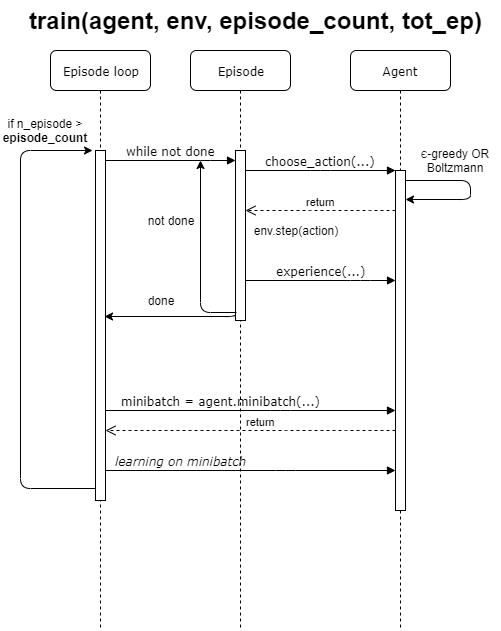
\includegraphics[width=.7\textwidth]{../src/img/Q7.png}
\end{center}

Ci-dessus, un diagramme de séquence simplifié de l'entraînement d'un Agent.

\subsubsection{Question 8 -- Target Network}

\end{document}
